\renewcommand{\thechapter}{\Roman{chapter}}
\chapter[]{METHODOLOGY}
\renewcommand{\thechapter}{\arabic{chapter}}
\begingroup
\fontsize{12pt}{\baselineskip}\selectfont
\section{Data Gathering}
	Training a descriptive model effectively necessitates a large-scale, high-fidelity dataset that pairs geometric representations with semantic natural language. However, unlike 2D image-captioning domains, the 3D CAD landscape suffers from a significant scarcity of standardized, human-readable annotations. To address this sparsity, a comprehensive acquisition framework was developed to ingest raw geometric data, filter for quality, and semantically enrich samples through a hybrid HITL process. A summary of the dataset preprocessing steps can be seen in \autoref{fig:dataset-acquisition-and-filtering-flowchart} below.
	\begin{figure}[H]
		\centering
		\includegraphics[width=0.6\linewidth]{"../Images/DATASET ACQUISITION AND FILTERING FLOWCHART"}
		\caption{Dataset acquisition and filtering flowchart.}
		\label{fig:dataset-acquisition-and-filtering-flowchart}
	\end{figure}
	
	\subsection{Dataset Source Selection}
		\begin{indentedblock}{4em}{0pt}
			Publicly available datasets for CAD file designs can be found on the internet. One prominent example is the ABC dataset, which consists of over one million unannotated STEP files derived from Onshape \parencite{abc_dataset_koch}. Another is the Fusion 360 Gallery, a dataset of free user-submitted designs with design timeline \parencite{fusion_dataset_karl}, and Text2CAD, which hosts around 170,000 CAD models with 660,000 natural language annotations ranging from short descriptions to detailed explanations \parencite{text2cad_khan}. Other sources include free 3D/CAD design websites such as GrabCAD and TraceParts, which contain various CAD objects not found in compiled datasets. A comparative summary for the sources listed above is contained in \autoref{tab:dataset-comparison-table} below.
			
			\skiplines{1}
			
			\begin{table}[H]
				\centering
				\footnotesize % significantly reduces font size to save vertical space
				\begin{tblr}{
						width=\linewidth, % Forces table to be as wide as the page
						colspec={
							Q[c,m,1.5cm]  
							Q[c,m,1.5cm]  
							X[2,c,m]    
							X[1.5,c,m]   
							X[1.5,c,m]    %
						},
						hlines,
						vlines,
						cells={valign=m, halign=l}, 
						rowsep=2pt 
					}
					\textbf{Source} & \textbf{Type} & \textbf{Summary} & \textbf{Advantages} & \textbf{Disadvantages} \\
					
					TraceParts & Online Library & Mfr-verified standard parts (bolts, gears, bearings). & High-fidelity geometry; ISO/DIN compliant. & Limited to standard hardware; requires scraping. \\
					
					GrabCAD & Online Library & 6M+ user files & High diversity of complex/creative designs. & Inconsistent quality; non-manifold geometry. \\ 
					
					Text2CAD & Dataset & Annotated CAD files with text-geometry pairs. & Ready-to-use labels; strictly organized. & Lower complexity than industry files. \\
					
					Fusion 360 & Dataset & Designs exported with assembly timelines. & Includes reconstruction history (timelines). & Proprietary format; inconsistent exports. \\
					ABC & Dataset & 1M+ unlabelled B-Rep files from Onshape. & Massive scale; robust topology for pre-training. & No semantic labels; contains "garbage" data. \\
					
				\end{tblr}
				\caption{Comparison of CAD Dataset Sources.}
				\label{tab:dataset-comparison-table}
			\end{table} 
			
			Based on the analysis detailed in \autoref{tab:dataset-comparison-table}, this paper will utilize a combination of CAD designs contained in Text2CAD as well as other online sources such as the ABC dataset and TraceParts. This combination ensures a balance between labeled semantic data (Text2CAD) and high-fidelity geometric variety (TraceParts). To help minimize discrepancies between annotations of several different datasets, a standard for annotation format mimicking the existing annotations in the Text2CAD dataset will be used.
			
		\end{indentedblock}

	\subsection{Dataset Preprocessing}
		\subsubsection{Dataset Filtering}
			\begin{indentedblock}{4em}{0pt}
				Before training, the dataset undergoes a rigorous analysis to eliminate rare or low-quality CAD designs that could destabilize the model. The filtering process is divided into two distinct stages. The first stage is \textbf{Class and Format Standardization}, implemented using PythonOCC. The script scans the raw data to enforce domain relevance by discarding any files not listed in the target object whitelist (e.g., excluding rare CAD designs and broken/corrupted files). Valid JSON-based CAD files are then automatically converted to STEP format using the OpenCascade library, while other unrecognizable formats are purged from the dataset.
				
				The next stage focuses on \textbf{Manifold Validation}. Since raw STEP files frequently contain disjointed surfaces or unstitched faces, a "water-tight" topological check is enforced, Using volumetric analysis (Volume $> 0$), any file containing open shells or non-manifold geometry is explicitly discarded. This initial geometric sanitation prevents invalid outliers from polluting the training signal, ensuring that the model only learns from physically realizable 3D objects.
				
				\skiplines{1}
	
				The second stage addresses statistical robustness by identifying and pruning \textit{long-tail} categories, or more specifically, classes containing fewer than 100 unique geometric instances. This threshold is critical for preventing model overfitting. Deep learning models often resort to memorization rather than generalization when handling classes with insufficient sample sizes \parencite{deep_learning_goodfellow}. As demonstrated by \textcite{generalization_zhang}, neural networks possess the capacity to fit arbitrary noise; in the absence of large-scale data constraints, they tend to memorize specific training instances rather than extracting abstract rules. This phenomenon leads to \textit{shortcut learning}, where the model identifies objects via spurious noise patterns or texture statistics instead of meaningful topological features \parencites{shortcut_learning_geirhos}{memorization_arpit}. 
				
				\skiplines{1}
				
				Furthermore, recent studies indicate that this vulnerability is exacerbated in high-variability datasets. Research by \textcite{memorization_effect_you} demonstrates that machine learning models struggle significantly to identify low-occurrence classes where the "class pattern" breaks due to high intra-class variance. By enforcing a minimum threshold of 100 instances, we ensure that every semantic category (e.g., \texttt{GEAR}, \texttt{BRACKET}) possesses sufficient geometric variance to force the Transformer to learn a generalized representation of the object type, rather than memorizing a handful of outliers.
				
			\end{indentedblock}
	
		\subsubsection{Dataset Standardization and Annotation Format}
			\begin{indentedblock}{4em}{0pt}
				The next preprocessing step involves designing an annotation standard for the unannotated CAD dataset sources to ensure homogeneity with the pre-annotated Text2CAD dataset through a multi-stage standardization and formatting pipeline. The pipeline standardizes varied input structures into a consistent, unified representation matching the multi-level description schema of the Text2CAD dataset.
				
				\skiplines{1}
				
				Data sourced from TraceParts often contains descriptive but non-standardized filenames (e.g., \textit{"Hexagon\_Head\_Screw\_ISO4017\_M8.stp"}). To extract the functional class, a \textbf{Hierarchical Regex Parser} is employed. The parser utilizes a dictionary of domain-specific keywords to map CAD files into general, high-level categories to ensure accurate annotation. The mapping logic follows a precedence order specified below to resolve ambiguities:
				
				\skiplines{1}
				
				\begin{enumerate}
					\item \textbf{Standard Extraction:} Strings containing ISO/DIN codes (e.g., "ISO 4017") are mapped immediately to their corresponding standard object family (e.g., \texttt{FASTENER}). This is done to exploit the rigorous standardization inherent in industrial engineering; parts explicitly labeled with international standards (ISO, DIN, ANSI) possess a verified, unambiguous functional identity, allowing them to serve as "Ground Truth" anchors for the classifier with near-100\% label confidence.
					
					\item \textbf{Morphological Keyword Search:} If no standard code is found, the parser scans for morphological roots. For example, filenames containing "gear", "pinion", or "worm" are all mapped to the class \texttt{GEAR} to simplify the manual annotation step.
					
					\item \textbf{Exclusion Logic:} To prevent misclassification of assemblies, filenames containing "Assy" or "Assembly" are flagged and excluded from the single-part classification dataset, as assembly CAD files s inherently represent composite systems containing multiple distinct components (e.g., a gearbox comprising shafts, bearings, and housings). Including these files would introduce label ambiguity, as a single input graph would correspond to multiple conflicting functional classes, which is outside the research's scope.
				\end{enumerate}
				
				Finally, while the hierarchical schema structure is retained for compatibility, the semantic objective of the annotation fields is redefined. Instead of describing the steps required to generate the object, the multi-level schema is used to categorize annotations of the same object based on their level of detail. \autoref{tab:annotation-level-table} below shows the defined annotation levels with an example for each level.
				
				\begin{table}[H]
					\centering
					\footnotesize % Reduces font size to save vertical space
					\begin{tblr}{
							width=\linewidth, % Forces table to use full page width
							colspec={
								Q[l,m,1.6cm]   % Level: Fixed, narrow
								X[1.25,l,m]     % Scope: Flexible, narrow-medium
								X[2.2,l,m]     % Definition: Flexible, medium
								X[3.5,l,m]     % Example: Flexible, widest
							},
							hlines,
							vlines,
							cells={valign=m},   % Vertically center all text
							rowsep=3pt          % Tightens vertical padding
						}
						\textbf{Level} & \textbf{Scope} & \textbf{Definition} & \textbf{Example Annotation} \\
						
						\textbf{Level 1 \newline (Abstract)} 
						& \textbf{Functional \newline Category} 
						& Identifies semantic class and primary application. Useful for high-level retrieval. 
						& "A standard metallic \textbf{fastener} designed for high-torque applications." \\
						
						\textbf{Level 2 \newline (Concrete)} 
						& \textbf{Morphological \newline Description} 
						& Describes visual geometry and topological features (shape types, head styles) without specific dimensions. 
						& "A \textbf{hexagonal-head bolt} featuring a partially threaded cylindrical shaft and a chamfered tip, with no washer face." \\
						
						\textbf{Level 3 \newline (Detailed)} 
						& \textbf{Parametric \newline Specification} 
						& Provides precise constraints, dimensions, and standard designations required for reconstruction. 
						& "An \textbf{ISO 4014 Hex Bolt} with a nominal thread diameter of \textbf{8mm} (M8), a total shaft length of \textbf{40mm}, and a thread pitch of 1.25mm." \\
						
					\end{tblr}
					\caption{Proposed Hierarchical Annotation Levels for Parametric Captioning}
					\label{tab:annotation-level-table}
				\end{table}
				
			\end{indentedblock}
					
		\subsubsection{Annotation Validation using BERTScore and Inter-Rater Reliability}
			\begin{indentedblock}{4em}{0pt}
				Since the dataset is comprised of multiple sources, with most lacking the necessary descriptive texts, an additional annotation step is needed. Unlike simple classification, generating natural language descriptions requires high-fidelity textual data that automated processes cannot fully synthesize. To extend the dataset beyond the pre-annotated Text2CAD samples, a \textbf{Human-in-the-Loop (HITL)} annotation pipeline is employed. Unlike simple filtering, this process utilizes \textbf{BERTScore} \parencite{bertscore_zhang} as a semantic validation metric to guide the manual annotation process, ensuring that new descriptions align stylistically with the established Text2CAD annotation schema specified in \autoref{tab:annotation-level-table}.
			
				\skiplines{1}
			
				The initial step includes writing manual annotations for each unannotated dataset entries which are validated by domain experts. The captions are designed to accurately describe the unlabelled geometric files (e.g., from TraceParts) with varying levels of detail. To maintain consistency, annotators follow a strict syntactic template derived from the Text2CAD dataset e.g. \textit{"[Functional Component] with [Geometric Features] and [Dimensions]."} This ensures that the training data remains uniform across different sources. 
				
				\skiplines{1}
				
				To validate the quality of the human-generated descriptions, a blind cross-verification study was conducted. A senior domain expert will be assigned to review a random sample of $N=500$ annotated descriptions, rating them as either "Compliant" or "Non-Compliant" based on the style guide. The consistency of this quality control process was measured using \textbf{Inter-Rater Reliability (IRR)}, specifically \textbf{Cohen's Kappa ($\kappa$)} \parencite{kappa_cohen}. This metric was chosen over simple percent agreement to robustly account for the possibility of chance agreement, with a target threshold of $\kappa > 0.80$ established to certify the dataset's reliability for training the transformer model \parencite{kappa_landis}.
			\end{indentedblock}
			
% --- SECTION 3.2 ---
\section{Model Design}
\label{sec:model-design}
	This research proposes a novel \textit{Hierarchical Dual-Stream Tokenizer} designed specifically to address the non-Euclidean nature of B-Rep (Boundary Representation) data. Unlike standard Natural Language Processing (NLP) tokenizers that treat input as a continuous 1D string which relies on the assumption that positional proximity equals semantic relationship, the proposed method treats the STEP file as a \textbf{topological graph}. This distinction is critical as in raw B-Rep data, geometric entities that are physically adjacent (e.g., two faces sharing an edge) may be defined thousands of lines apart in the ASCII file structure. Therefore, the data must be \textbf{normalized} to remove coordinate invariance, \textbf{compressed} to eliminate redundant entity definitions, and \textbf{linearized} via a deterministic graph traversal to preserve local geometric neighborhoods before ingestion.
	
% --- SUBSECTION 3.2.1 ---
	\subsection{Tokenizer Architecture}
		\begin{indentedblock}{4em}{0pt}
			
			The tokenization pipeline consists of four distinct stages designed to ensure geometric invariance and computational efficiency. The overarching goal of the tokenizer is to bridge the \textit{semantic gap} between the low-level mathematical definitions of CAD surfaces and the high-level semantic reasoning required by the Transformer. However, a standard tokenizer faces several issues when parsing STEP files. One such issue is \textit{semantic fragmentation} of high-precision floating-point coordinates into meaningless sub-word units (e.g., splitting "10.125" into separate tokens "10", ".", "12", "5"), which destroys the numerical magnitude required for geometric reasoning \parencite{deepcad_wu}. Second, standard sequential processing fails to capture the \textit{non-local graph topology} inherent in B-Rep data; in a raw STEP file, spatially adjacent geometric features are often defined thousands of lines apart and linked only by arbitrary reference IDs (e.g., \#243), creating long-range dependencies that exhaust the finite attention span of standard Transformer models \parencite{deepcad_wu}. The proposed architecture aims to solve these limitations by integrating \textbf{Complex-Valued Embeddings} \parencite{trabelsi_2017_deep} and \textbf{Rotary Positional Encodings} \parencite{su_2023_roformer}. This allows the model to inherently encode geometric rotation and magnitude within the latent space, preserving topological fidelity without relying on reconstruction history. \autoref{fig:tokenizer-pipeline} below shows an overview of the tokenizer architecture. 
		
			\begin{figure}[H]
				\centering
				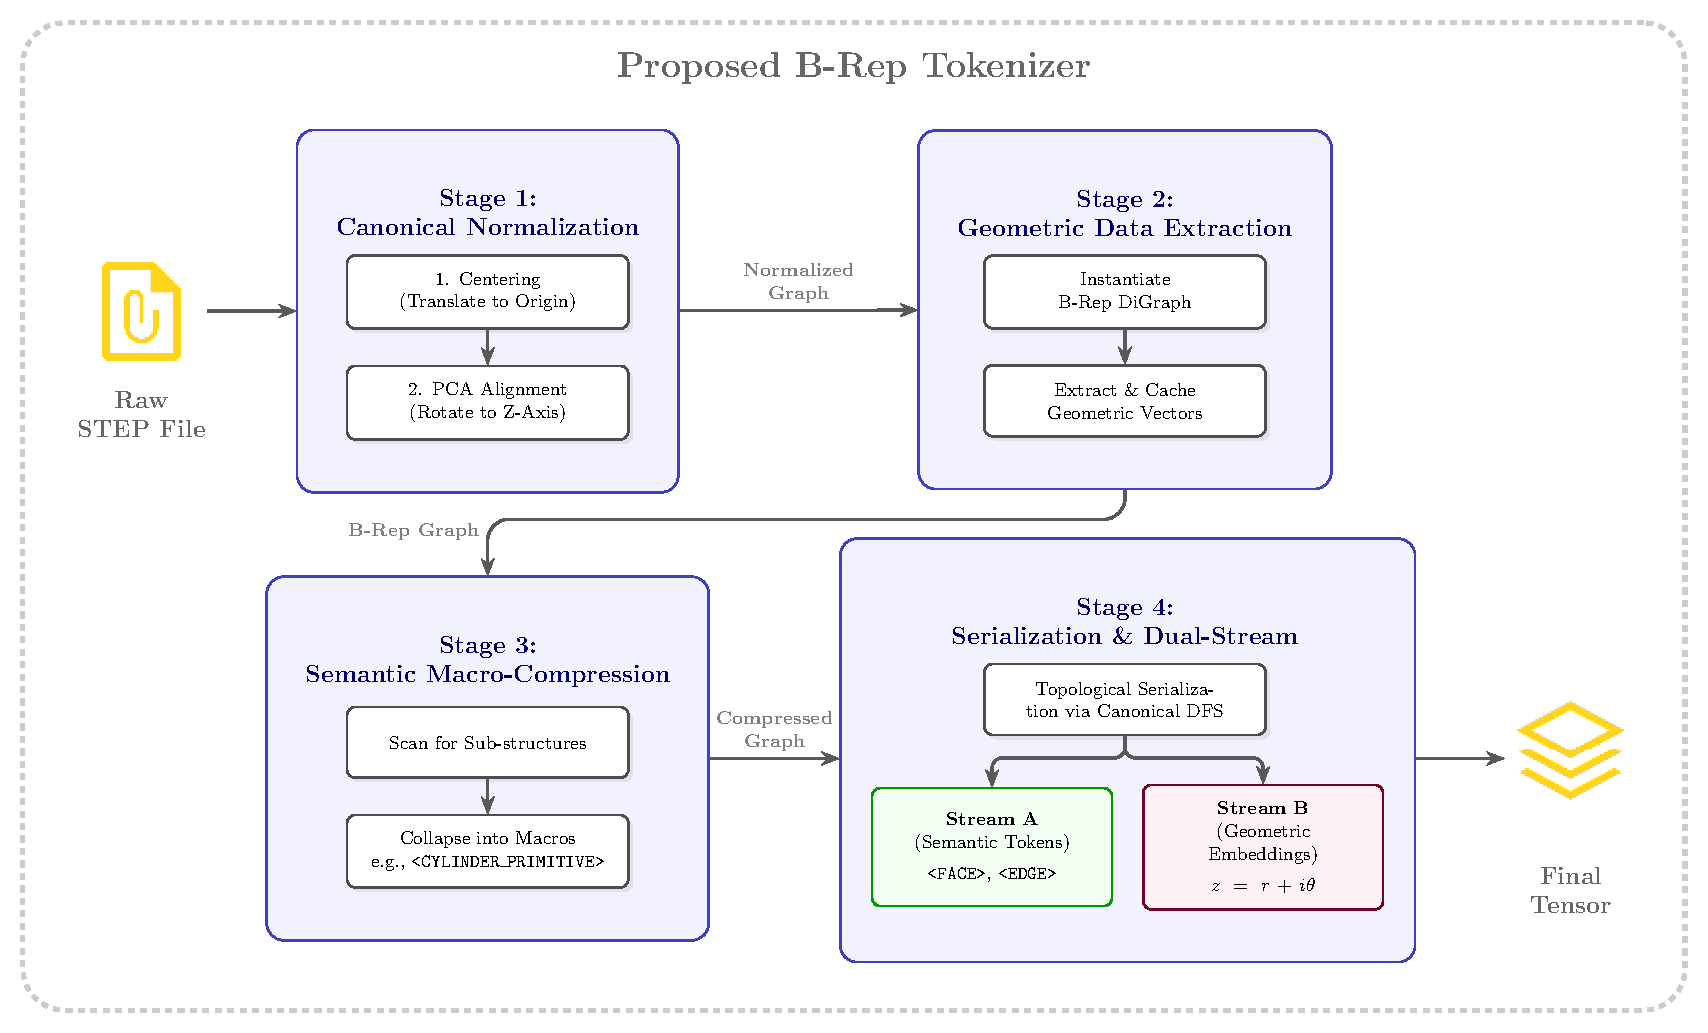
\includegraphics[width=0.8\linewidth]{../Images/TikZ/TOKENIZER.pdf} 
				\caption{The proposed four-stage tokenization pipeline.}
				\label{fig:tokenizer-pipeline}
			\end{figure}
			
		\end{indentedblock}
			\subsubsection{Stage 1: Semantic Macro-Compression}
				\begin{indentedblock}{4em}{0pt}
					Raw STEP files exhibit extreme verbosity, where semantically simple manufacturing features are explicitly defined by dozens of constituent low-level topological entities. One example of this is objects such as a "Through-Hole" is represented not as a feature, but as a \texttt{CYLINDRICAL\_SURFACE} connected to two \texttt{CIRCLE} edges, which are further linked to \texttt{VERTEX\_POINT} definitions. As noted in foundational generative studies, such excessive sequence length dilutes the attention mechanism's ability to model global structure, often leading to convergence failure on complex assemblies \parencite{deepcad_wu}. Furthermore, flat B-Rep graphs fail to capture the hierarchical nature of mechanical assemblies, necessitating a multi-level graph representation to efficiently encode topological adjacency \parencite{colligan_2022_hierarchical}.
					
					To mitigate this, a \textbf{Semantic Graph Contraction} algorithm is applied as a pre-tokenization step. A rule-based parser performs subgraph isomorphism checks to identify and compress known topological patterns into smaller, niche tokens. For instance, a \texttt{CYLINDRICAL\_SURFACE} bounded by two \texttt{CIRCLE} edges is fused into a single macro-node \texttt{<CYLINDER\_PRIMITIVE>}. Similarly, adjacent chains of tangential \texttt{B\_SPLINE\_SURFACE} patches are aggregated into \texttt{<FILLET\_CHAIN>} macros. This heuristic reduces the generated sequence length while retaining the semantic essence of the geometry, effectively increasing the model's receptive field and allowing the Transformer to reason about feature-level relationships rather than low-level surface connectivity.
					
					
				\end{indentedblock}
		
			\subsubsection{Stage 2: Canonical Geometric Normalization}
				\begin{indentedblock}{4em}{0pt}
					Standard STEP coordinates are sensitive to global positioning, i.e. a single mechanical component defined at coordinate $(0,0,0)$ might generate different token sequences than the same component translated to $(100,100,100)$. A sufficiently accurate model must achieve translational and rotational invariance, meaning that its output is not dependent on the translation and rotation of the input data \parencites{medical_imaging_li}{rotational_invariance_muaz}. To achieve this, the B-Rep graph undergoes a rigorous \textbf{Canonical Alignment} process. This reduces the dimensionality of the learning manifold by ensuring that all semantically identical objects occupy the same region in the input vector space \parencite{deepcad_wu}. The normalization pipeline is implemented using three mathematical transformations described below:
					\begin{enumerate}
						\item \textbf{Centroid Subtraction (Translation Invariance):} The geometric center of mass $\mu$ is computed across all control points $P = \{p_1, p_2, ..., p_N\}$ in the solid. All vertices are then translated such that the centroid aligns with the global origin:
						\begin{equation}
							p'_i = p_i - \frac{1}{N}\sum_{j=1}^{N} p_j
						\end{equation}
						
						\item \textbf{PCA Alignment (Rotation Invariance):} To align the geometry with a consistent canonical orientation, Principal Component Analysis (PCA) is performed on the vertex cloud \parencite{alignment_chaouch}. We compute the covariance matrix $\Sigma$:
						\begin{equation}
							\Sigma = \frac{1}{N} \sum_{i=1}^{N} p'_i (p'_i)^T
						\end{equation}
						The eigenvectors $v_1, v_2, v_3$ of $\Sigma$ (corresponding to the largest to smallest eigenvalues) represent the primary, secondary, and tertiary axes of variance. The entire geometry is rotated via a matrix $R = [v_1, v_2, v_3]$ such that the axis of greatest variance (e.g., the length of a screw) aligns with the global $z$-axis.
						
						\item \textbf{Ambiguity Resolution:} A standard PCA alignment suffers from sign ambiguity (the "180-degree flip" problem), where a bolt might be aligned pointing Up or Down randomly. To resolve this, a deterministic "heavy-bottom" rule is enforced: if the density of points in the negative $z$ half-space is lower than the positive half-space, the axis is flipped ($z' = -z$). This ensures consistent orientation across the dataset \parencite{3d_model_retrieval_vranic}.
					\end{enumerate}
				\end{indentedblock}
		
			\subsubsection{Stage 3: Topological Linearization (Canonical DFS)}
				\begin{indentedblock}{4em}{0pt}
					Since Transformers utilize positional encoding to interpret sequence order, the serialization of the B-Rep graph must be strictly deterministic. A standard Depth-First Search (DFS) is insufficient because it is sensitive to the stochastic permutation of entity identifiers in the STEP file (e.g., visiting \texttt{\#10=FACE} before \texttt{\#20=FACE} purely based on arbitrary ID assignment). This introduces \textbf{Graph Isomorphism Ambiguity}: two geometrically identical cubes could produce entirely different token sequences if their internal numbering differs, forcing the model to waste capacity learning to ignore these permutations \parencite{deepcad_wu}.
					
					Resolving the ambiguity requires the implementation of a \textbf{Canonical DFS} traversal. The algorithm introduces a strict ordering constraint at every branch of the graph, where for any parent node $N_p$ (e.g., a \texttt{SHELL}) with a set of child nodes $C = \{c_1, c_2, ..., c_k\}$ (e.g., \texttt{FACES}), the children are strictly sorted based on a geometric invariant function vector $\mathbf{f}(c)$ before the traversal continues. The ordering logic is defined as:
					
					\begin{equation}
						\text{Order}(C) = \text{sort}_{\downarrow}\left( \{ \mathbf{f}(c) \mid c \in C \} \right)
					\end{equation}
					
					In this research, the invariant function $\mathbf{f}(c)$ is designed to be invariant to both rigid body rotation and file re-indexing by utilizing a \textbf{Hierarchical Sorting Key} which consists of 3 parts:
					\begin{itemize}
						\item \textbf{Primary Key ($k_1$):} \textit{Geometric Magnitude}. For Topological Faces, this is the \textbf{Surface Area}; for Edges, it is the \textbf{Curve Length}. This ensures that large, dominant features (like the main body of a housing) appear early in the sequence, providing a stable "context" for the attention mechanism.
						\item \textbf{Secondary Key ($k_2$):} \textit{Centroid Distance}. To resolve symmetries (tie-breaking), we calculate the Euclidean distance from the entity's centroid to the global origin $(0,0,0)$. 
						\item \textbf{Tertiary Key ($k_3$):} \textit{Topological Degree}. The number of connected edges/loops.
					\end{itemize}
					
					\paragraph{Handling Symmetries (Tie-Breaking)}
						In cases of perfect symmetry (e.g., a Cube where all 6 faces have identical Area and Centroid Distance), a deterministic fallback is required. The fallback procedure utilizes the principal axis alignment from Stage 2: faces are sorted by their centroid's $Z, Y, X$ coordinates respectively. This guarantees that a specific 3D geometry yields an \textit{identical} token sequence regardless of the permutation of entity IDs in the raw file \parencite{colligan_2022_hierarchical}. 
%						\autoref{fig:canonical-dfs} illustrates the proposed DFS algorithm.
				
%					\begin{figure}[htbp]
%						\centering
%						% PLACEHOLDER FOR DIAGRAM B (Canonical DFS Visualization)
%						\includegraphics[width=0.8\linewidth]{example-image-b} 
%						\caption{Comparison of Standard DFS vs. Canonical DFS. By sorting child nodes based on geometric properties (e.g., area) rather than file ID, the tokenizer guarantees a deterministic sequence for identical geometries.}
%						\label{fig:canonical-dfs}
%					\end{figure}
				\end{indentedblock}
			
			\subsubsection{Stage 4: Complex-Valued Dual-Stream Encoding}
			\begin{indentedblock}{4em}{0pt}
				To preserve high-fidelity precision (e.g., NURBS weights) without bloating the discrete vocabulary, a Dual-Stream architecture is used. The tokenizer emits two parallel streams for every step $t$:
				\begin{itemize}
					\item \textbf{Stream A (Semantic Tokens):} Discrete integers representing the categorical type of entity (e.g., \texttt{<FACE>}, \texttt{<NURBS\_CURVE>}).
					\item \textbf{Stream B (Geometric Embeddings):} A 128-dimensional \textbf{Complex-Valued Vector} encoding the shape parameters.
				\end{itemize}
			\end{indentedblock}
			
			\begin{indentedblock}{4em}{0pt}
				The complex vector $v \in \mathbb{C}^{64}$ encodes the geometry as $z = r + i\theta$. The real part $r$ represents scale-invariant magnitudes (e.g., radius, edge length), while the imaginary part $\theta$ encodes the relative orientation. This formulation is inspired by Euler's formula ($e^{i\theta}$), allowing the model to perform rotation operations purely through phase shifts in the complex domain.
			\end{indentedblock}
		
	% --- SUBSECTION 3.2.2 ---
	\subsection{Model Parameters}
		\begin{indentedblock}{4em}{0pt}
			The core model is a Transformer Encoder based on the BERT architecture \parencite{bert_devlin}, modified to accept the Dual-Stream input.
			
			\begin{itemize}
				\item \textbf{Embedding Dimension ($d_{model}$):} 512. The discrete tokens are embedded into $\mathbb{R}^{512}$, and the 128-dim complex geometric vectors are projected via a Multi-Layer Perceptron (MLP) to $\mathbb{R}^{512}$ before summation.
				\item \textbf{Attention Heads:} 8 Parallel heads.
				\item \textbf{Layers:} 12 Encoder blocks.
				\item \textbf{Context Window:} 2048 tokens.
				\item \textbf{Feed-Forward Network:} GELU activation with a dimension of 2048.
			\end{itemize}
			
			The selection of these hyperparameters is governed by the specific trade-offs inherent to B-Rep graph learning. While modern LLMs often utilize dimensions upwards of 4096, CAD syntax has a significantly smaller vocabulary size ($<1000$ unique structural tokens). A dimension of $d_{model}=512$ was chosen to prevent overfitting on this sparse vocabulary while providing sufficient manifold capacity to represent the fused Dual-Stream input. 
			
			The choice of 12 layers aligns with the hierarchical nature of boundary representation. Lower layers ($L_{1-4}$) are tasked with learning local topological syntax (e.g., edge continuity), intermediate layers ($L_{5-8}$) aggregate these into feature-level representations (e.g., pockets, bosses), and upper layers ($L_{9-12}$) extract high-level semantic class information.
			
			Standard BERT implementations utilize a 512-token window. However, B-Rep graphs—even after the proposed Macro-Compression—exhibit long-range dependencies where a face defined at token $T_1$ may reference a surface defined at token $T_{1000}$. A window of 2048 tokens was empirically selected to encompass the complete topological graph of 95\% of the dataset samples without necessitating destructive truncation.
		\end{indentedblock}
		
		\subsubsection{Geometry-Infused Attention Mechanism}
		\begin{indentedblock}{4em}{0pt}
			Unlike standard NLP Transformers where the attention score is derived solely from semantic word embeddings, the proposed architecture employs a \textbf{Geometry-Infused Attention} mechanism. This mechanism is responsible for synthesizing the Dual-Stream output from the tokenizer into a unified representation.
			
			The input to the attention layer for the $i$-th token is defined as the fusion of the semantic and geometric streams:
			\begin{equation}
				X_i = \text{Embed}(T_i) + \text{MLP}(V_i)
			\end{equation}
			Where $T_i$ is the discrete semantic token (e.g., \texttt{<FACE>}) and $V_i$ is the 128-dimensional complex geometric vector. The Multi-Layer Perceptron (MLP) acts as a bridge, projecting the continuous geometric manifold into the semantic model dimension $d_{model}$.
			
			\paragraph{Geometric Rotary Positional Integration}
			To strictly enforce the rotational invariance defined in the methodology, the model utilizes a modified version of Rotary Positional Embeddings (RoPE). The "Phase" component ($\theta$) of the complex geometric input $V_i$ is directly mapped to the rotation of the Query ($Q$) and Key ($K$) vectors in the attention calculation:
			\begin{equation}
				\text{Attention}(Q, K, V) = \text{softmax}\left(\frac{(R_{\theta_i}Q)(R_{\theta_j}K)^T}{\sqrt{d_k}}\right)V
			\end{equation}
			Here, $R_{\theta}$ represents the rotation matrix derived from the tokenizer's complex input. This ensures that the attention score between two CAD entities depends not only on their semantic type but also on their \textbf{relative geometric orientation}. For example, a \texttt{SCREW} entity will attend strongly to a \texttt{HOLE} entity only if their orientation vectors (Normal vectors) are aligned (i.e., the relative rotation $\Delta\theta \approx 0$), thereby embedding physical assembly logic directly into the attention weights.
		\end{indentedblock}

	\subsubsection{Classification Head}
		\begin{indentedblock}{4em}{0pt}
			The final representation is extracted via Global Average Pooling across the sequence length, condensing the topological graph into a single latent vector $Z_{graph} \in \mathbb{R}^{512}$. This vector is passed to a softmax classifier to predict the functional category of the mechanical part, adhering to the class schema defined in the data gathering phase.
		\end{indentedblock}

% --- SECTION 3.3 ---
\section{Training and Backtesting}

	\subsection{Training Setup}
		\begin{indentedblock}{4em}{0pt}
			The classification objective is optimized using \textbf{Categorical Cross-Entropy Loss}. This function penalizes the divergence between the predicted probability distribution $\hat{y}$ and the ground truth one-hot vector $y$. For a dataset of $N$ samples and $C$ classes, the loss $\mathcal{L}$ is defined as:
			
			\begin{equation}
				\mathcal{L} = -\frac{1}{N} \sum_{i=1}^{N} \sum_{c=1}^{C} y_{i,c} \log(\hat{y}_{i,c})
			\end{equation}
			
			Where $\hat{y}_{i,c}$ is the softmax probability output of the model for class $c$. The logarithmic nature of the loss function imposes a heavy penalty on confident but incorrect predictions, which is critical for distinguishing between visually similar CAD classes (e.g., distinguishing an ISO-4014 Bolt from an ISO-4017 Bolt based on subtle shaft length variations).
		\end{indentedblock}

	\subsection{Evaluation Metrics}
		\begin{indentedblock}{4em}{0pt}
			To validate the effectiveness of the proposed tokenizer, the model is evaluated on two fronts:
			\begin{enumerate}
				\item \textbf{Standard Classification Metrics:} Accuracy, Precision, Recall, and F1-Score on a held-out test set (20\% of the data).
				\item \textbf{Rotational Robustness Test:} A specialized test set is generated by applying random random $SO(3)$ rotations to the test data. The model's accuracy on this rotated set is compared to the baseline to verify the efficacy of the Canonical Alignment and Complex-Valued Embeddings.
			\end{enumerate}
		\end{indentedblock}
	
\endgroup